Determine the first five eigenvalues of the problem

$$u_{xxxx}+u_{xxx}=\lambda u_{xx},\;\; u(\pm2)=u_x(\pm2)=0,\;\; -2<x<2$$

and plot the corresponding eigenvectors.\\

\begin{solution}\renewcommand{\qedsymbol}{}\ \\
    Using the code developed below, we have the following five eigenvalues:

    $$e_1=-3.5268$$

    $$e_2=-4.4447$$

    $$e_3=-10.8290$$

    $$e_4=-14.4444$$

    $$e_5=-23.1561$$

    As such, we have the following plot of the eigenvectors:

    \begin{center}
        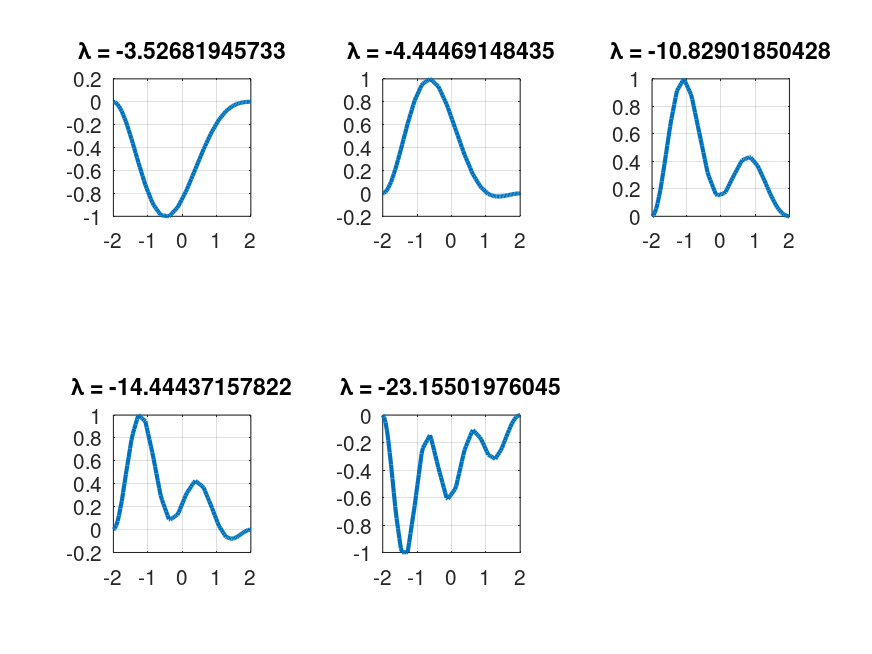
\includegraphics[scale=0.4]{problem14_1_evects.PNG}
    \end{center}

\end{solution}

\newpage
\lstinputlisting{problem14_1.m}
\newpage